\documentclass{beamer}
%\usepackage{beamerarticle}

\usepackage[ngerman]{babel}
\usepackage[utf8]{inputenc}
\usepackage[T1]{fontenc}
\usepackage{tikz}
\usetikzlibrary{positioning, arrows}
\usepackage{listings}
\usepackage{fancybox}
\usepackage{verbatim}

\usepackage{pifont}% http://ctan.org/pkg/pifont
\newcommand{\cmark}{\ding{51}}%
\newcommand{\xmark}{\ding{55}}%

\usetheme{Madrid}
\setbeamercovered{transparent}

\title[SWT-Praktikum]{Pr\"sentationen mit dem Paktet  Beamer}
\author{swp15.gkp}
\date{\today{}}
%\logo{\includegraphics[scale=0.25]{logo}}

\begin{document}
\begin{frame}
\center \huge \textbf{Kartenbasiertes Multiplayerspiel} \\
\center \huge \textbf{P U C M A N}
\end{frame}

\begin{frame}{Überblick}
\begin{itemize}
\item Der Prozess
\item Kartengenese
\end{itemize}
\end{frame}

\begin{frame}
\begin{figure}[htbp] 
  \centering
     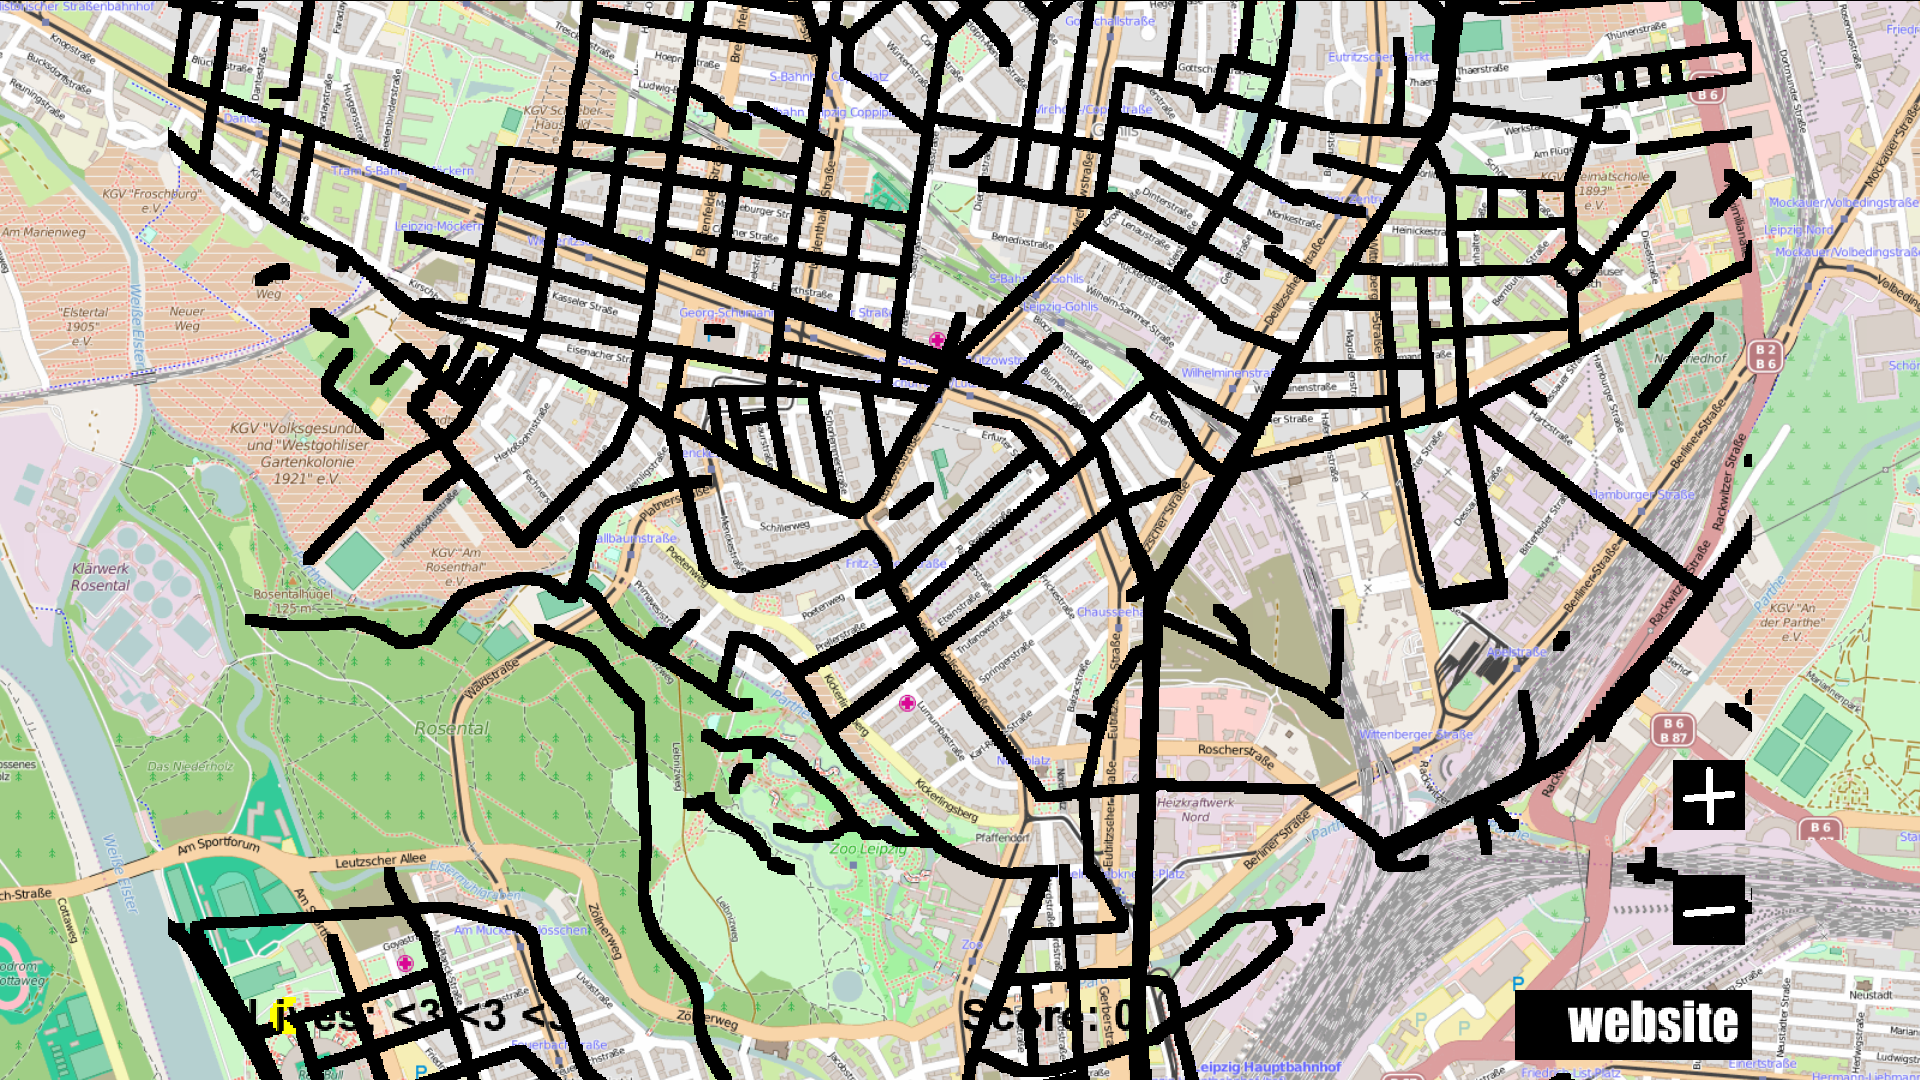
\includegraphics[width=1\textwidth]{03.png}
  \caption{Erstes Bild}
  \label{fig:Bild1}
\end{figure}

\end{frame}

\begin{frame}
\begin{figure}[htbp] 
  \centering
     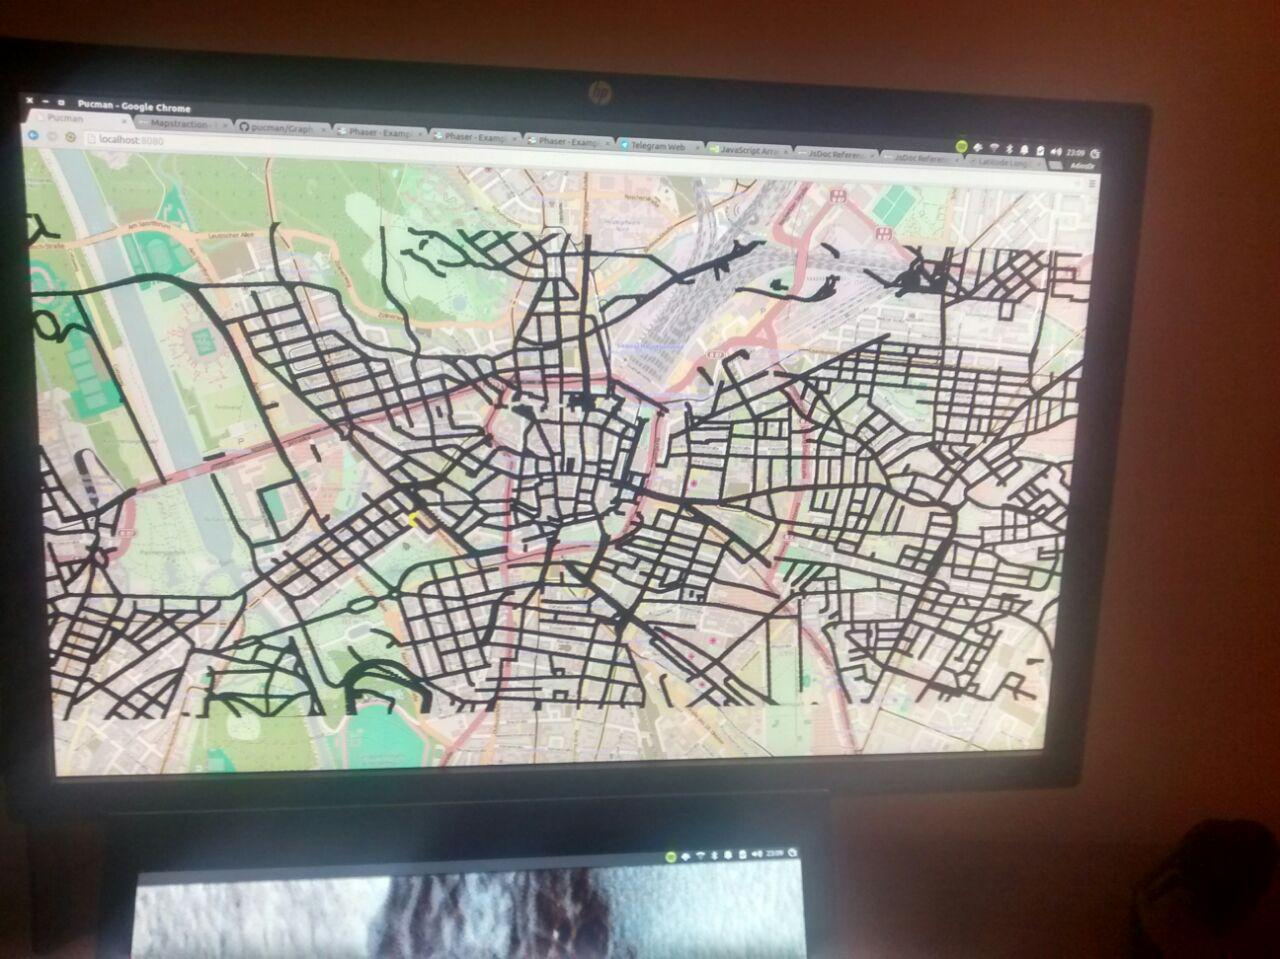
\includegraphics[width=1\textwidth]{05.jpg}
  \caption{Erstes Bild}
  \label{fig:Bild1}
\end{figure}

\end{frame}

\begin{frame}
\begin{figure}[htbp] 
  \centering
     
\includegraphics[width=1\textwidth]{06.jpg}
  \caption{Erstes Bild}
  \label{fig:Bild1}
\end{figure}

\end{frame}
\begin{frame}
\begin{figure}[htbp] 
  \centering
     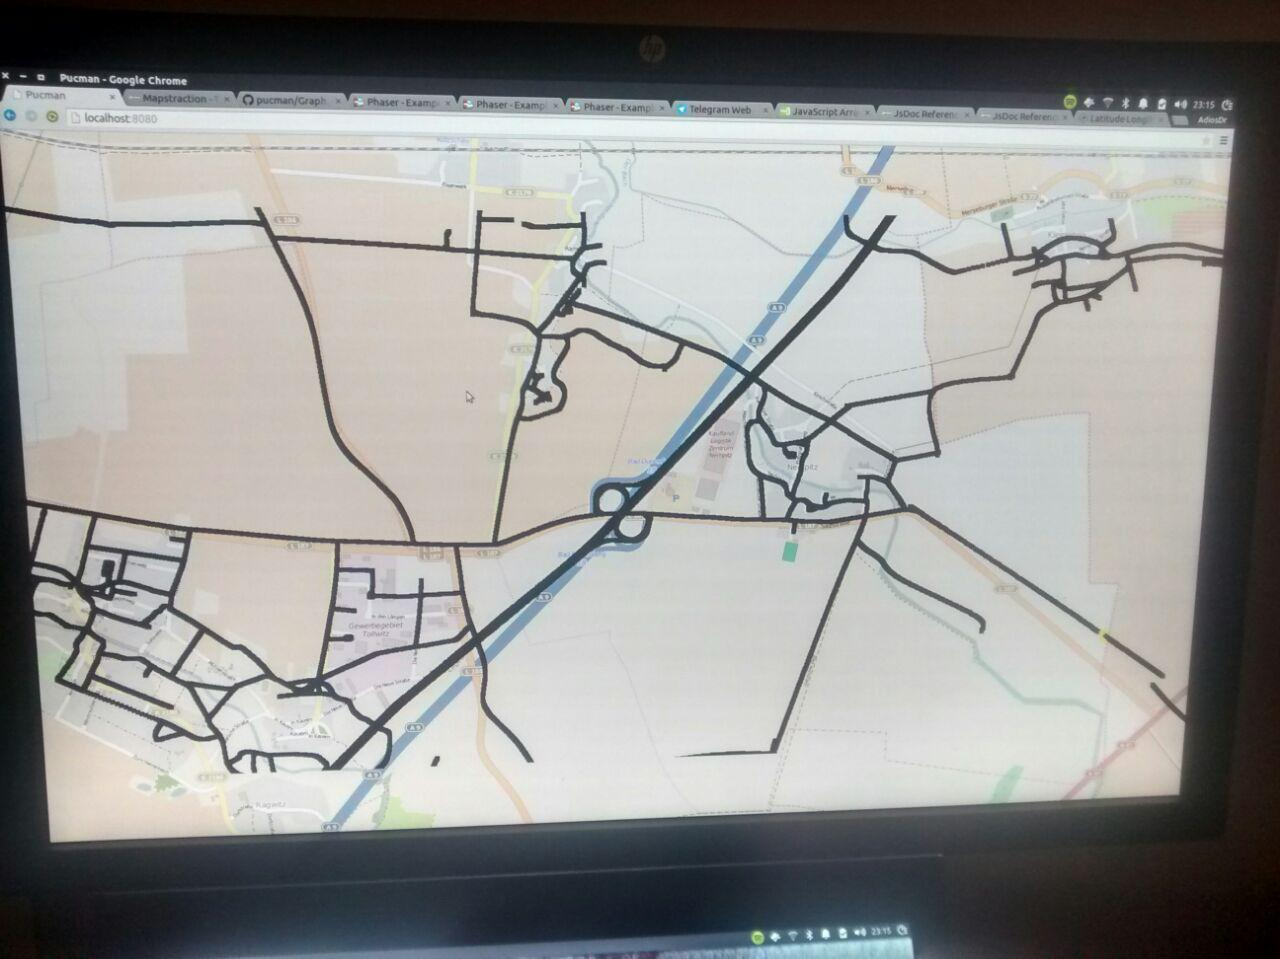
\includegraphics[width=1\textwidth]{07.jpg}
  \caption{Erstes Bild}
  \label{fig:Bild1}
\end{figure}

\end{frame}

\begin{frame}
\begin{figure}[htbp] 
  \centering
     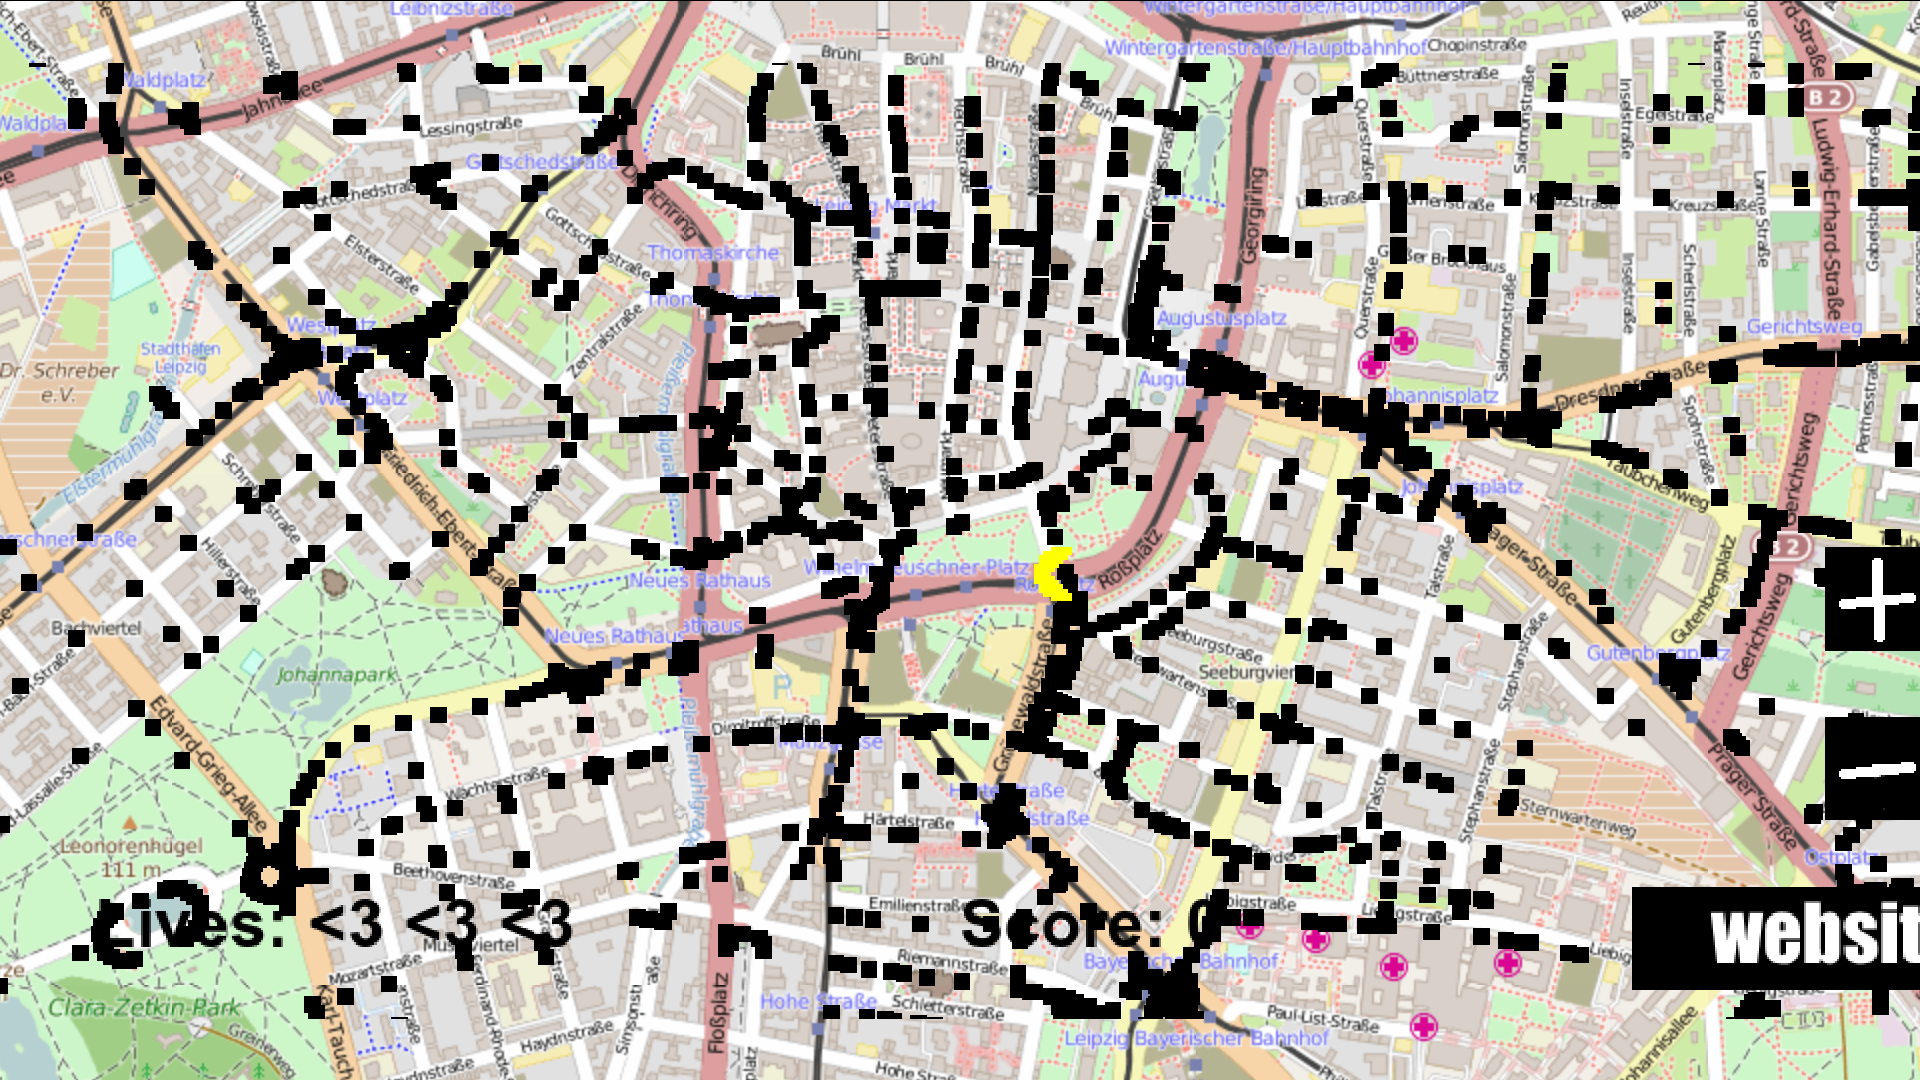
\includegraphics[width=1\textwidth]{04.png}
  \caption{Erstes Bild}
  \label{fig:Bild1}
\end{figure}

\end{frame}


\begin{frame}
\begin{figure}[htbp] 
  \centering
     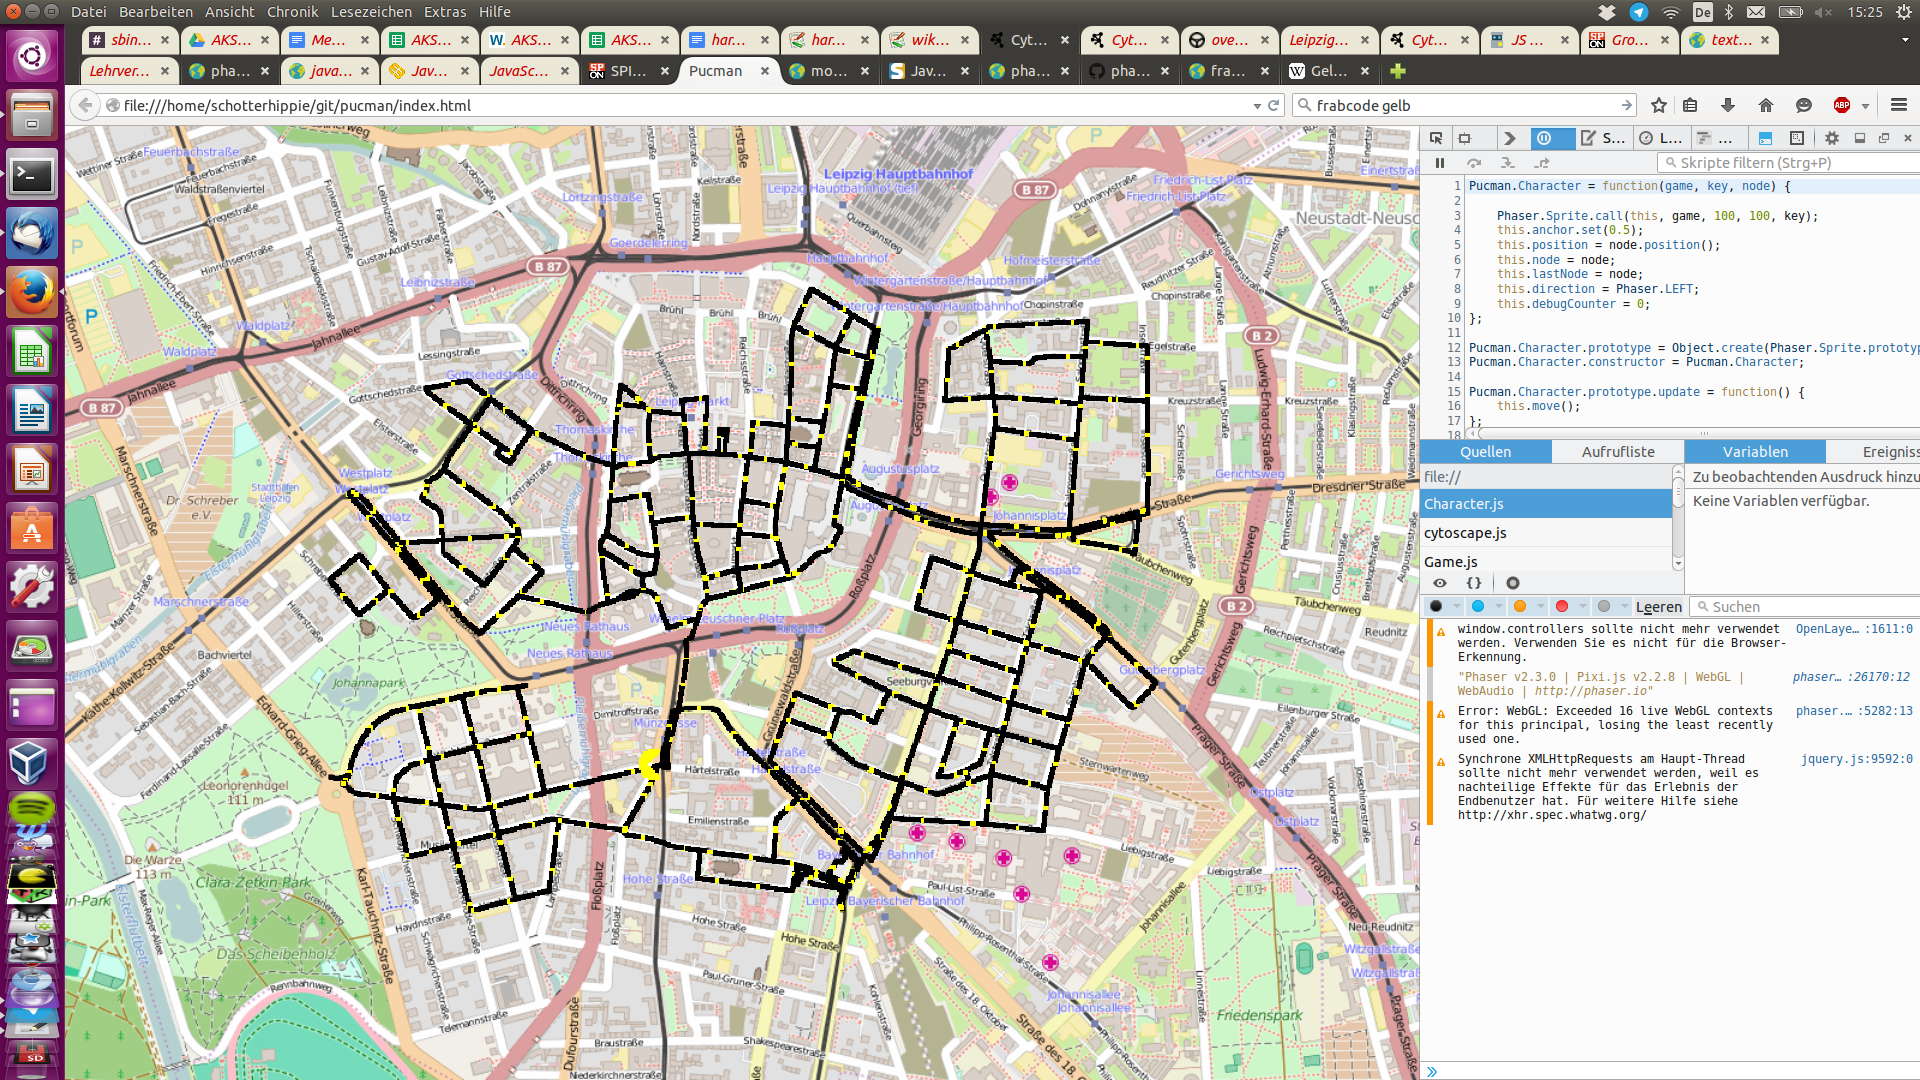
\includegraphics[width=1\textwidth]{01.png}
  \caption{Erstes Bild}
  \label{fig:Bild1}
\end{figure}
\end{frame}

\begin{frame}
\begin{figure}[htbp] 
  \centering
     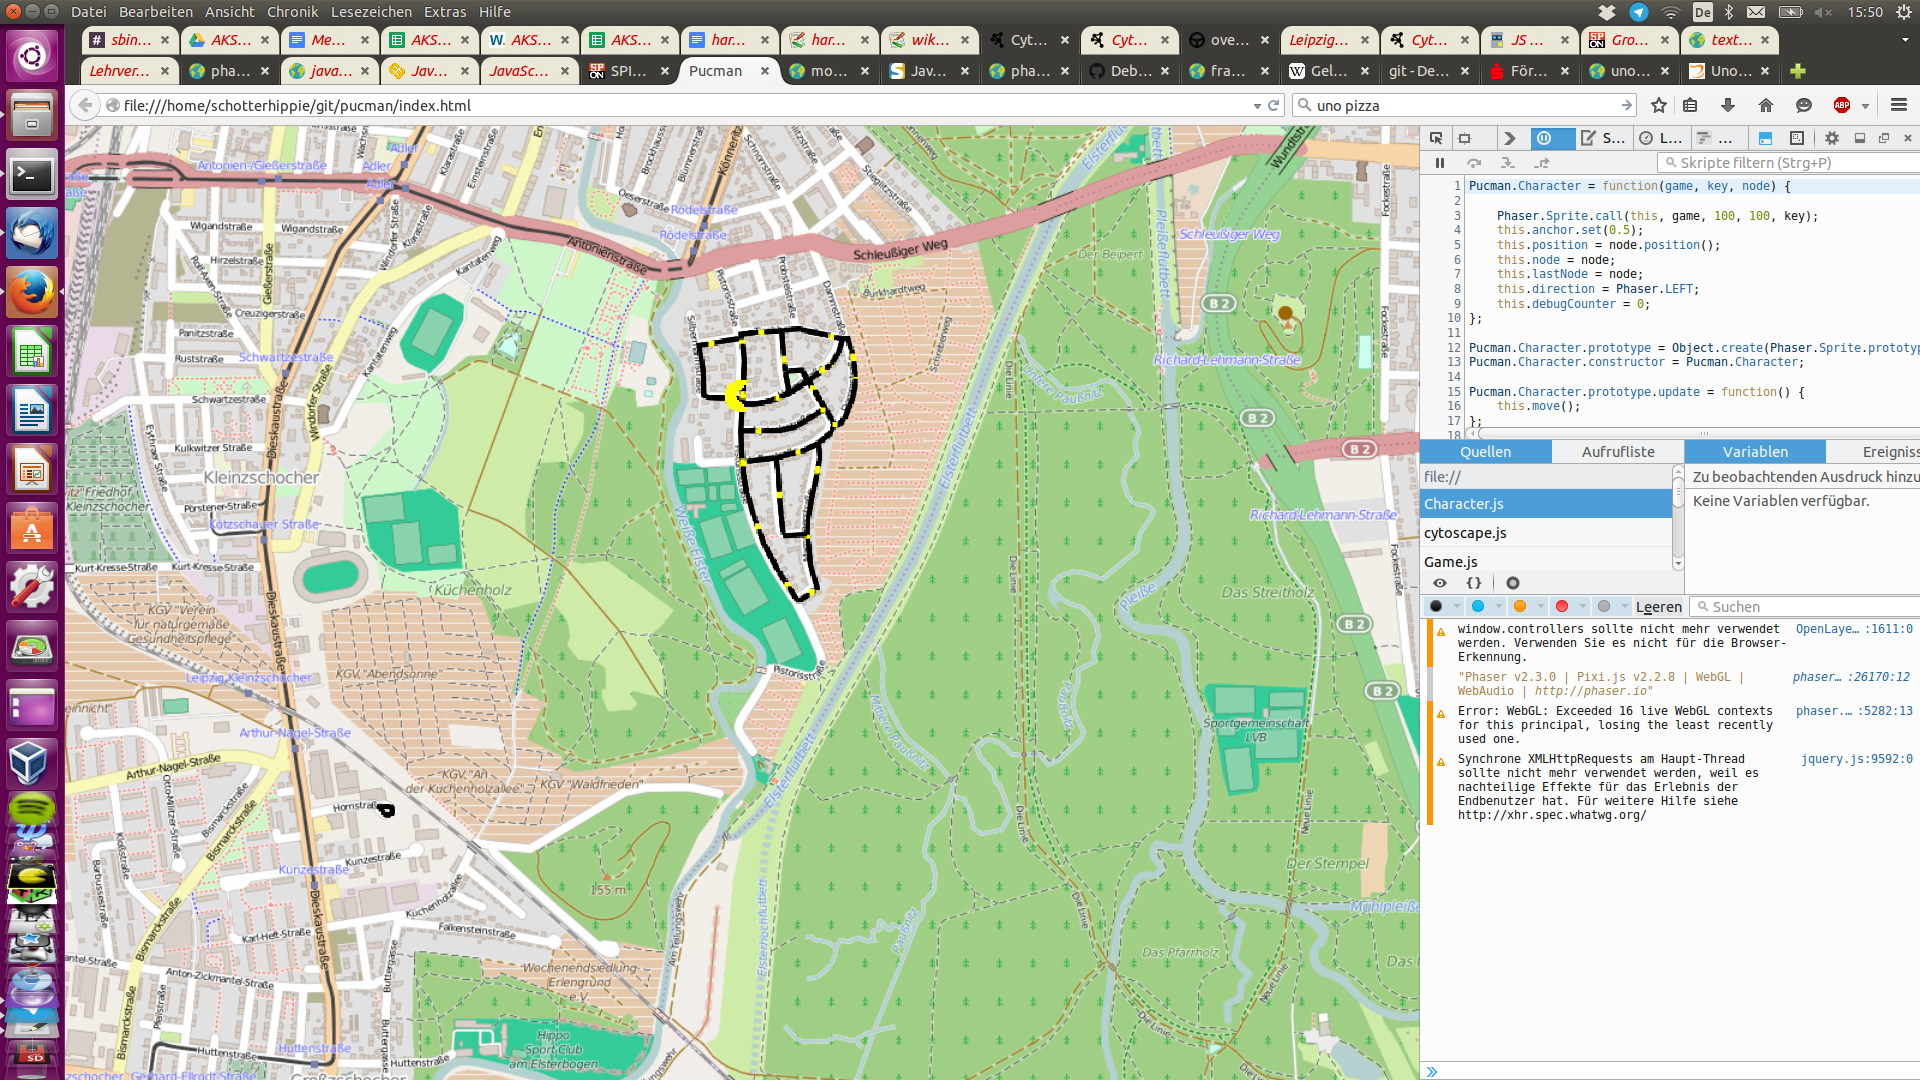
\includegraphics[width=1\textwidth]{02.png}
  \caption{Erstes Bild}
  \label{fig:Bild1}
\end{figure}

\end{frame}



\begin{frame}
\Huge \center \textbf{F R A G E N ?}
\end{frame}
\end{document}